%------------------------------------------------------------------------------
% Code
%------------------------------------------------------------------------------

% Command based on: https://tex.stackexchange.com/questions/266811/define-a-new-command-with-parameters-inside-newcommand
\newcommand{\codeName}[1]{\expandafter\newcommand\csname #1\endcsname{\inlineHs{#1}}}

% Used for showing what the blue-highlighted text is, in the reading notes section
\codeName{ExampleText}

% Defines commands to be used in poster and thesis

\newcommand{\swebokScalDef}{This seems to define ``usability
    testing'' with elements of functional and recovery testing}
\newcommand{\swebokElasRef}{only cites a single source
    \textbf{that doesn't contain the words ``elasticity'' or ``elastic''}!}

% for assets/code/example.tex...
\newcommand{\exampleCode}{\begin{codeSnippet}{haskell}{``MultiDefinitions'' (MultiDefn) Definition}{exampleCode}{https://github.com/JacquesCarette/Drasil/blob/051b9881a6417e51e818c6673c5eab0f48bd5af2/code/drasil-theory/lib/Theory/Drasil/MultiDefn.hs\#L45-L56}
-- | 'MultiDefn's are QDefinition factories, used for showing one or more ways
--   we can define a QDefinition.
data MultiDefn e = MultiDefn{
  -- | UID
  _rUid :: UID,
  -- | Underlying quantity it defines.
  _qd :: QuantityDict,
  -- | Explanation of the different ways we can define a quantity.
  _rDesc :: Sentence,
  -- | All possible ways we can define the related quantity.
  _rvs :: NE.NonEmpty (DefiningExpr e)
}
\end{codeSnippet}
}
\newcommand{\refExampleCode}{\Cref{lst:exampleCode}}

% for assets/code/examplePseudocode.tex...
\newcommand{\examplePseudocode}{\begin{pseudocode}{haskell}{Broken QuantityDict Chunk Retriever}{examplePseudocode}
retrieveQD :: UID -> ChunkDB -> Maybe QuantityDict
retrieveQD u cdb = do
    (Chunk expectedQd) <- lookup u cdb
    pure expectedQd
\end{pseudocode}
}
\newcommand{\refExamplePseudocode}{\Cref{lst:examplePseudocode}}

% for assets/code/mainInvalidInputTest.tex...
\newcommand{\mainInvalidInputTest}{\begin{codeSnippet}{python}{Tests for main with an invalid input file}{mainInvalidInputTest}{https://github.com/samm82/Drasil/blob/sysTests/code/stable/projectile/projectile_c_p_nol_b_u_v_d/src/python/test/Control_test.py\#L29-L53}
  # from https://stackoverflow.com/questions/54071312/how-to-pass-command-line-argument-from-pytest-to-code
  ## \brief Tests main with invalid input file
  # \par Types of Testing:
  # Dynamic Black-Box (Behavioural) Testing
  # Boundary Conditions
  # Default, Empty, Blank, Null, Zero, and None
  # Invalid, Wrong, Incorrect, and Garbage Data
  # Logic Flow Testing
  @mark.parametrize("filename", invalid_value_input_files)
  @mark.xfail
  def test_main_invalid(monkeypatch, filename):
      # from https://stackoverflow.com/questions/10840533/most-pythonic-way-to-delete-a-file-which-may-not-exist
      try:
          remove(output_filename)
      except OSError as e: # this would be "except OSError, e:" before Python 2.6
          if e.errno != ENOENT: # no such file or directory
              raise # re-raise exception if a different error occurred


      assert not path.exists(output_filename)


      with monkeypatch.context() as m:
          m.setattr(sys, 'argv', ['Control.py', str(Path("test/test_input") / f"{filename}.txt")])
          Control.main()
      
      assert not path.exists(output_filename)
\end{codeSnippet}
}
\newcommand{\refMainInvalidInputTest}{\Cref{lst:mainInvalidInputTest}}

% for assets/code/projManualViolationReq.tex...
\newcommand{\projManualViolationReq}{\begin{codeSnippet}{haskell}{\acs{projectile}'s manually created requirement for constraint violation behaviour}{projManualViolationReq}{https://github.com/JacquesCarette/Drasil/blob/afb6fb752b8364d2807ced7fc0c1dd6c6aba52b2/code/drasil-example/projectile/lib/Drasil/Projectile/Requirements.hs\#L31-L34}
verifyParamsDesc = foldlSent [S "Check the entered", plural inValue,
    S "to ensure that they do not exceed the" +:+. namedRef (datCon [] []) (plural datumConstraint),
    S "If any of the", plural inValue, S "are out of bounds" `sC`
    S "an", phrase errMsg, S "is displayed" `S.andThe` plural calculation, S "stop"]
\end{codeSnippet}
}
\newcommand{\refProjManualViolationReq}{\Cref{lst:projManualViolationReq}}

% for assets/code/projViolationChoice.tex...
\newcommand{\projViolationChoice}{\begin{codeSnippet}{haskell}{\acs{projectile}'s choice for constraint violation behaviour in code}{projViolationChoice}{https://github.com/JacquesCarette/Drasil/blob/afb6fb752b8364d2807ced7fc0c1dd6c6aba52b2/code/drasil-example/projectile/lib/Drasil/Projectile/Choices.hs\#L120}
    srsConstraints = makeConstraints Warning Warning,
\end{codeSnippet}
}
\newcommand{\refProjViolationChoice}{\Cref{lst:projViolationChoice}}

%------------------------------------------------------------------------------
% Graphs
%------------------------------------------------------------------------------

% Organization of files
\newcommand{\ExampleGraph}{
    \begin{figure*}
        \begin{subfigure}[b]{0.4\linewidth}
            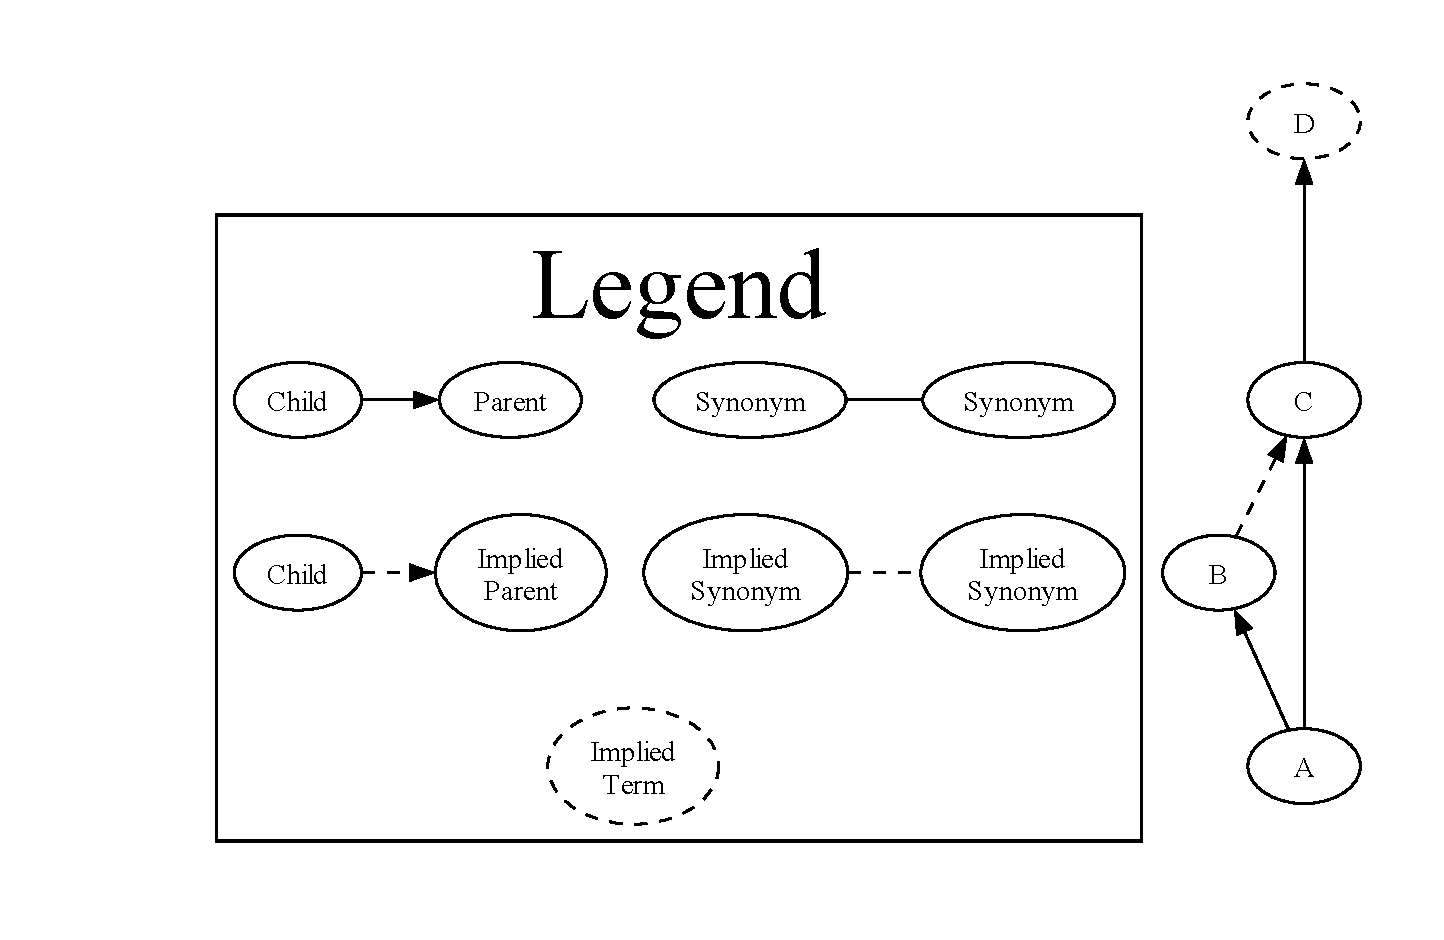
\includegraphics[width=\linewidth]{assets/graphs/ExampleGlossaryGraph.pdf}
            \caption{Graph from \Cref{tab:exampleGlossary}.}
            \label{fig:exampleGraph}
        \end{subfigure}
        \begin{subfigure}[b]{0.575\linewidth}
            \centering
            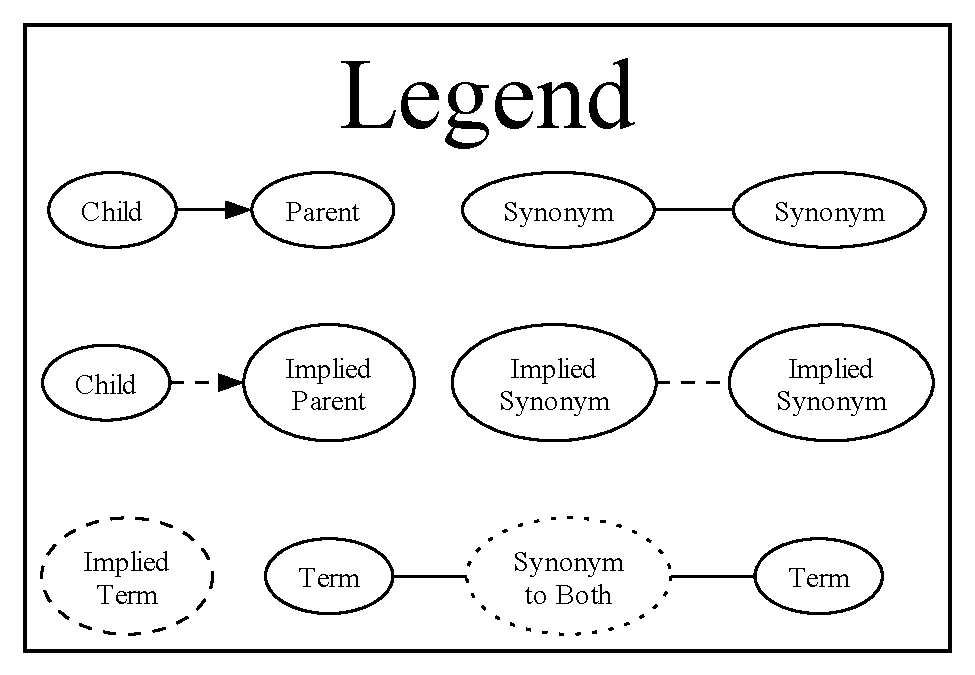
\includegraphics[width=\linewidth]{assets/graphs/manual/manualLegendNonSolidTerms.pdf}
            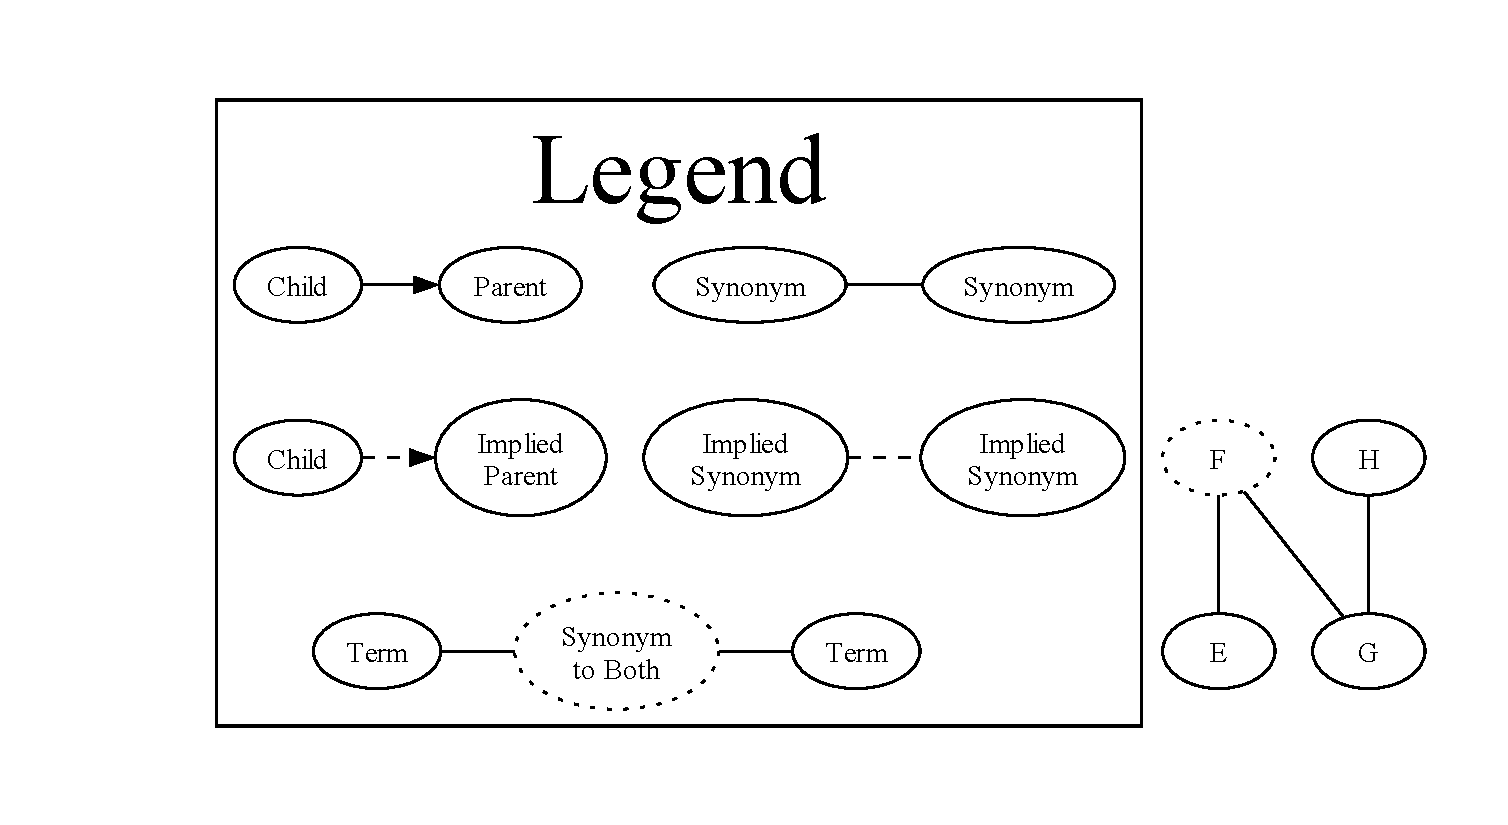
\includegraphics[width=0.85\linewidth]{assets/graphs/SynExampleGlossaryGraph.pdf}
            \caption{Graph from \Cref{tab:synExampleGlossary}.}
            \label{fig:synExampleGraph}
        \end{subfigure}
        \begin{subfigure}[b]{0.3\linewidth}
            \hspace{-1.35cm}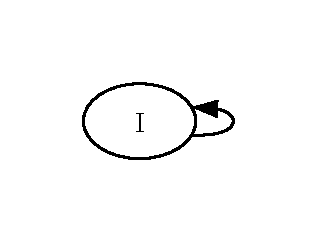
\includegraphics[width=1.3\linewidth]{assets/graphs/SelfExampleGlossaryGraph.pdf}
            \vspace{5mm}
            \caption{Graph generated from a .tex file containing a line starting with
                \texttt{I -> I}.}
            \label{fig:selfExampleGraph}
        \end{subfigure}
        \hfill
        \begin{subfigure}[b]{0.325\linewidth}
            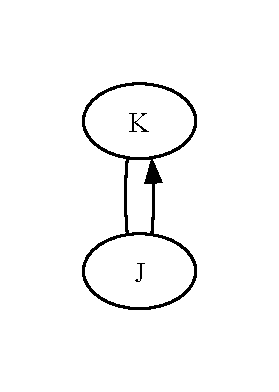
\includegraphics[width=1.1\linewidth]{assets/graphs/ParSynExampleGlossaryGraph.pdf}
            \caption{Graph generated from a .tex file containing a line starting with
                \texttt{J -> K} if J and K are synonyms.}
            \label{fig:parSynExampleGraph}
        \end{subfigure}
        \hfill
        \begin{subfigure}[b]{0.28\linewidth}
            \hspace{-2.05cm}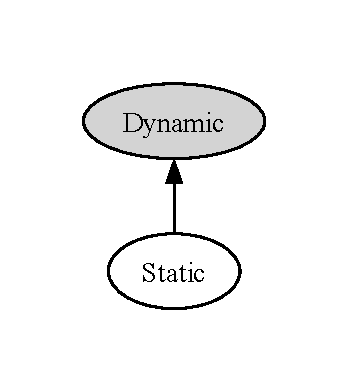
\includegraphics[width=1.5\linewidth]{assets/graphs/StaticExampleGlossaryGraph.pdf}
            \caption{Graph of static approaches showing that related dynamic approaches are colored gray.}
            \label{fig:staticExampleGraph}
        \end{subfigure}
        \caption{Example generated graphs.}
        \label{fig:exampleGraphs}
    \end{figure*}
}

\newcommand{\performanceGraph}{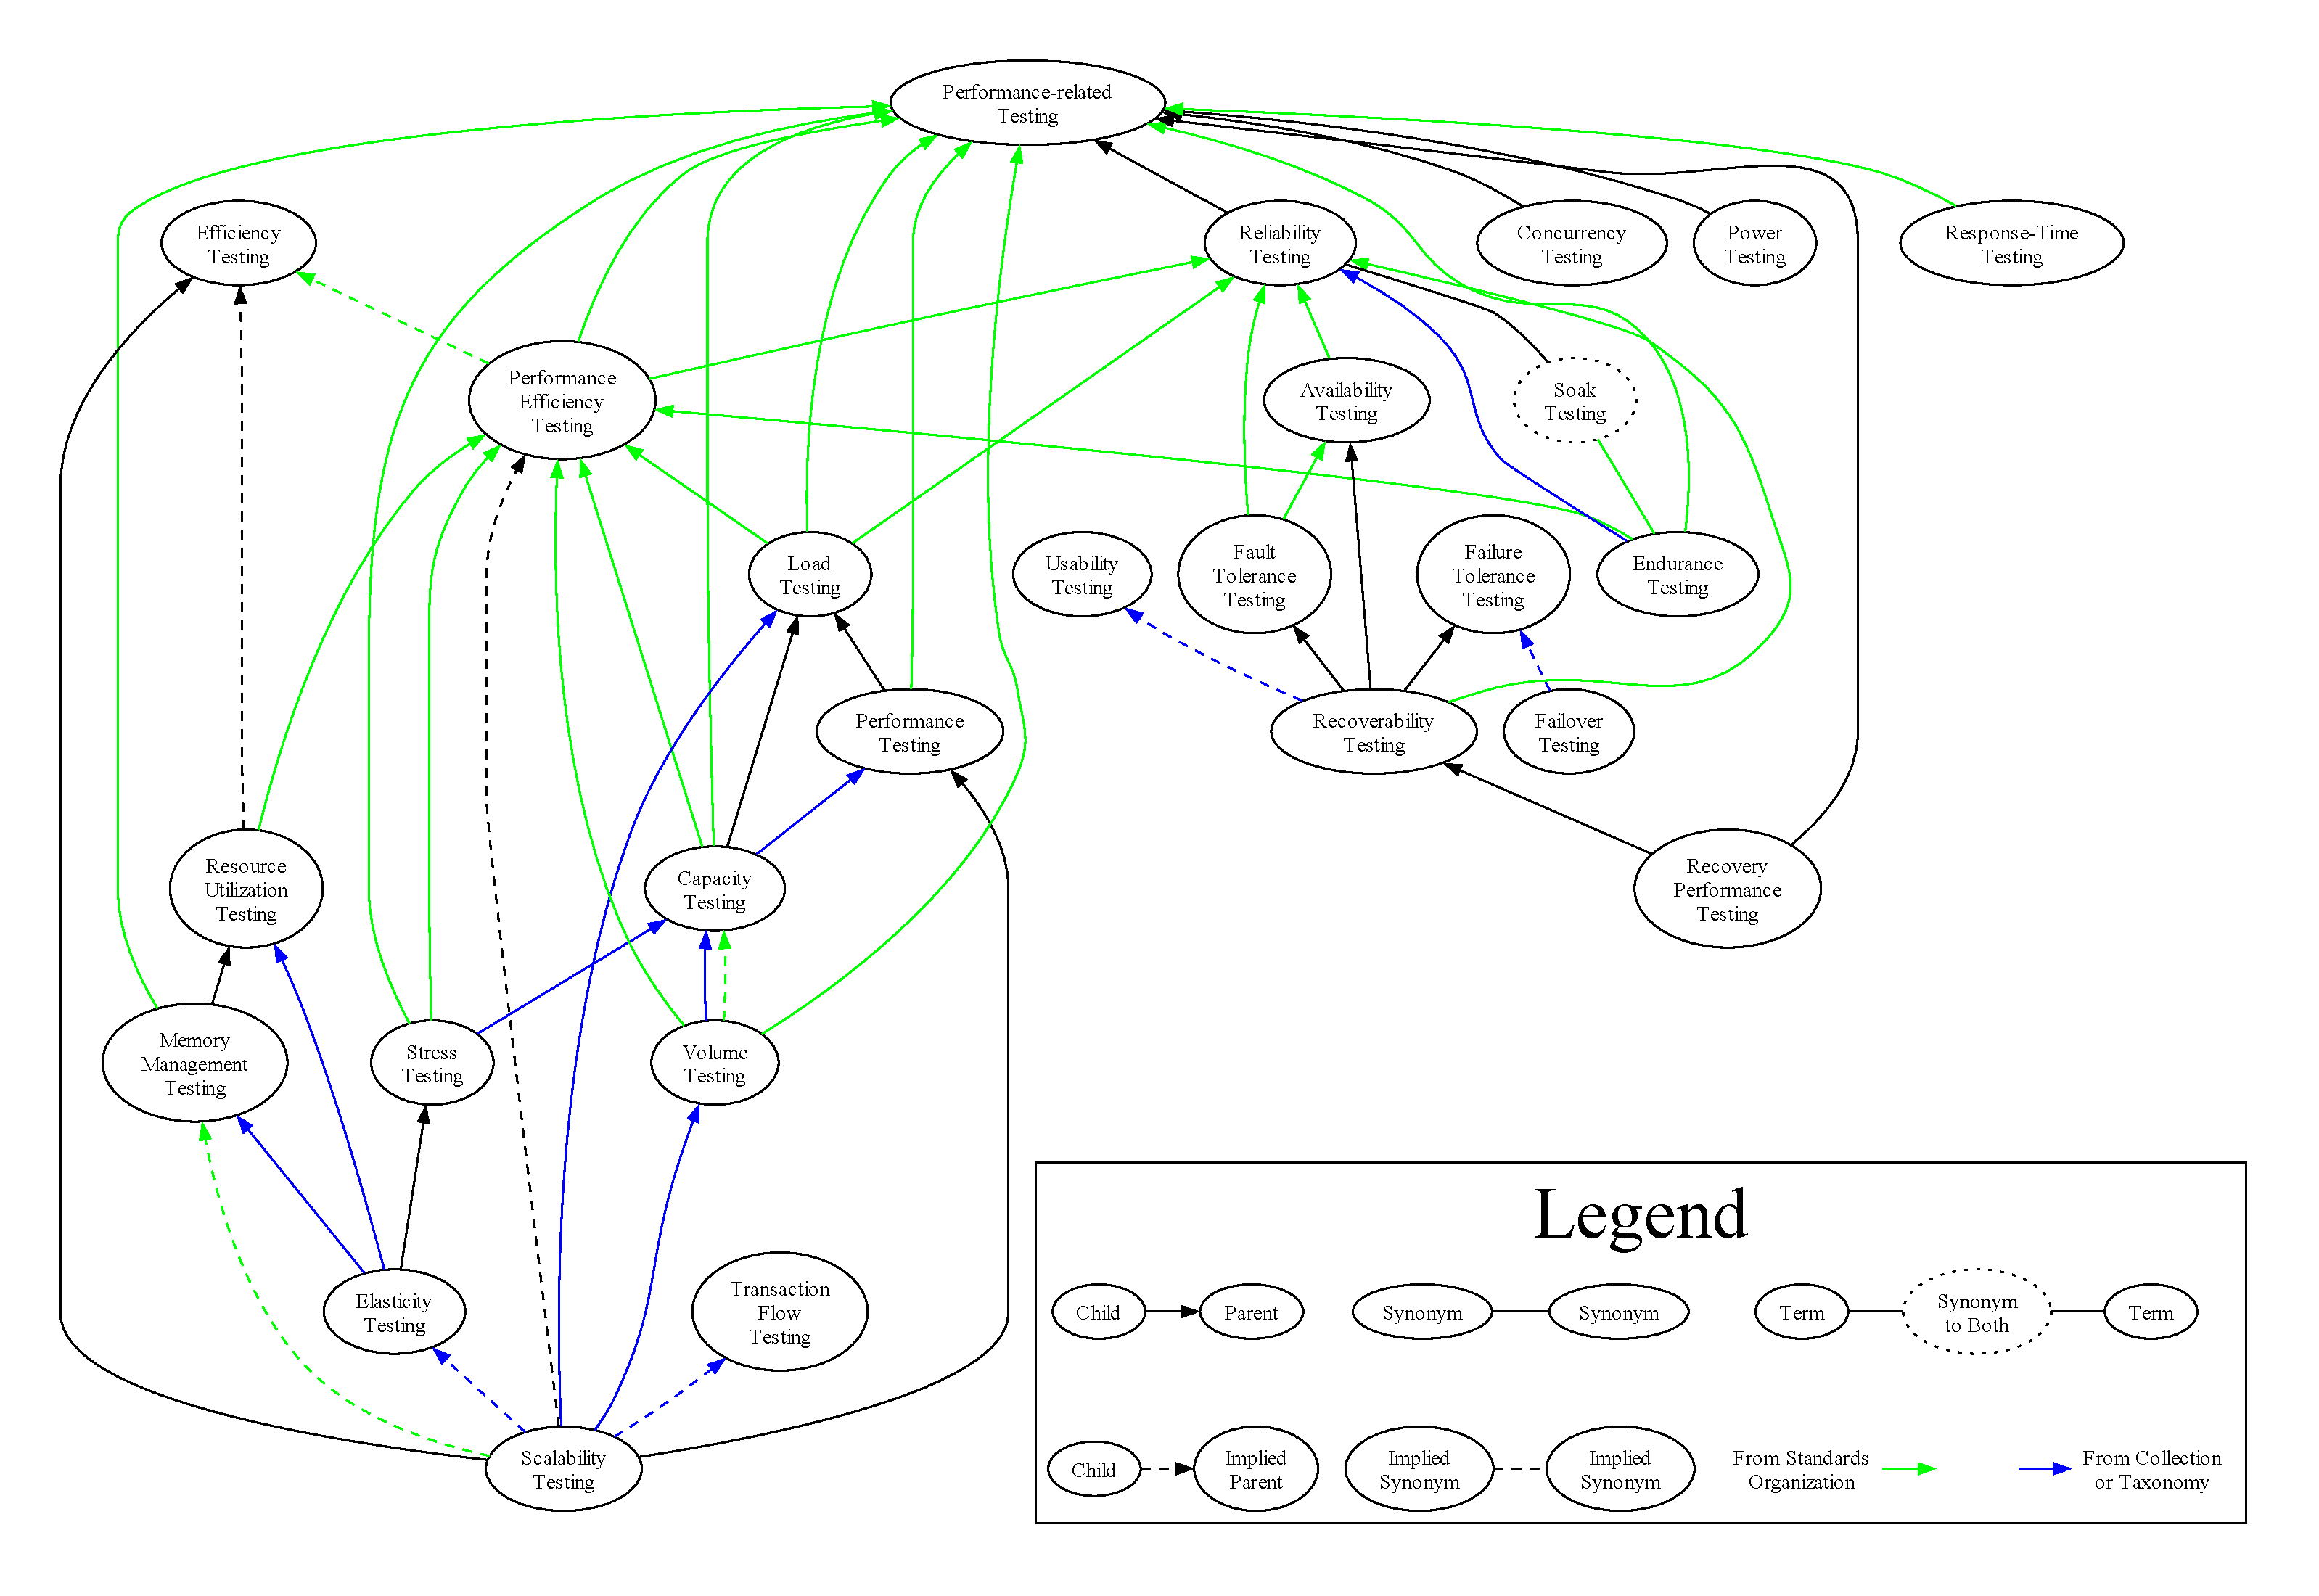
\includegraphics[width=0.8\linewidth]{assets/graphs/manual/performanceProposedGraph.pdf}}
\newcommand{\recoveryGraphCurrent}{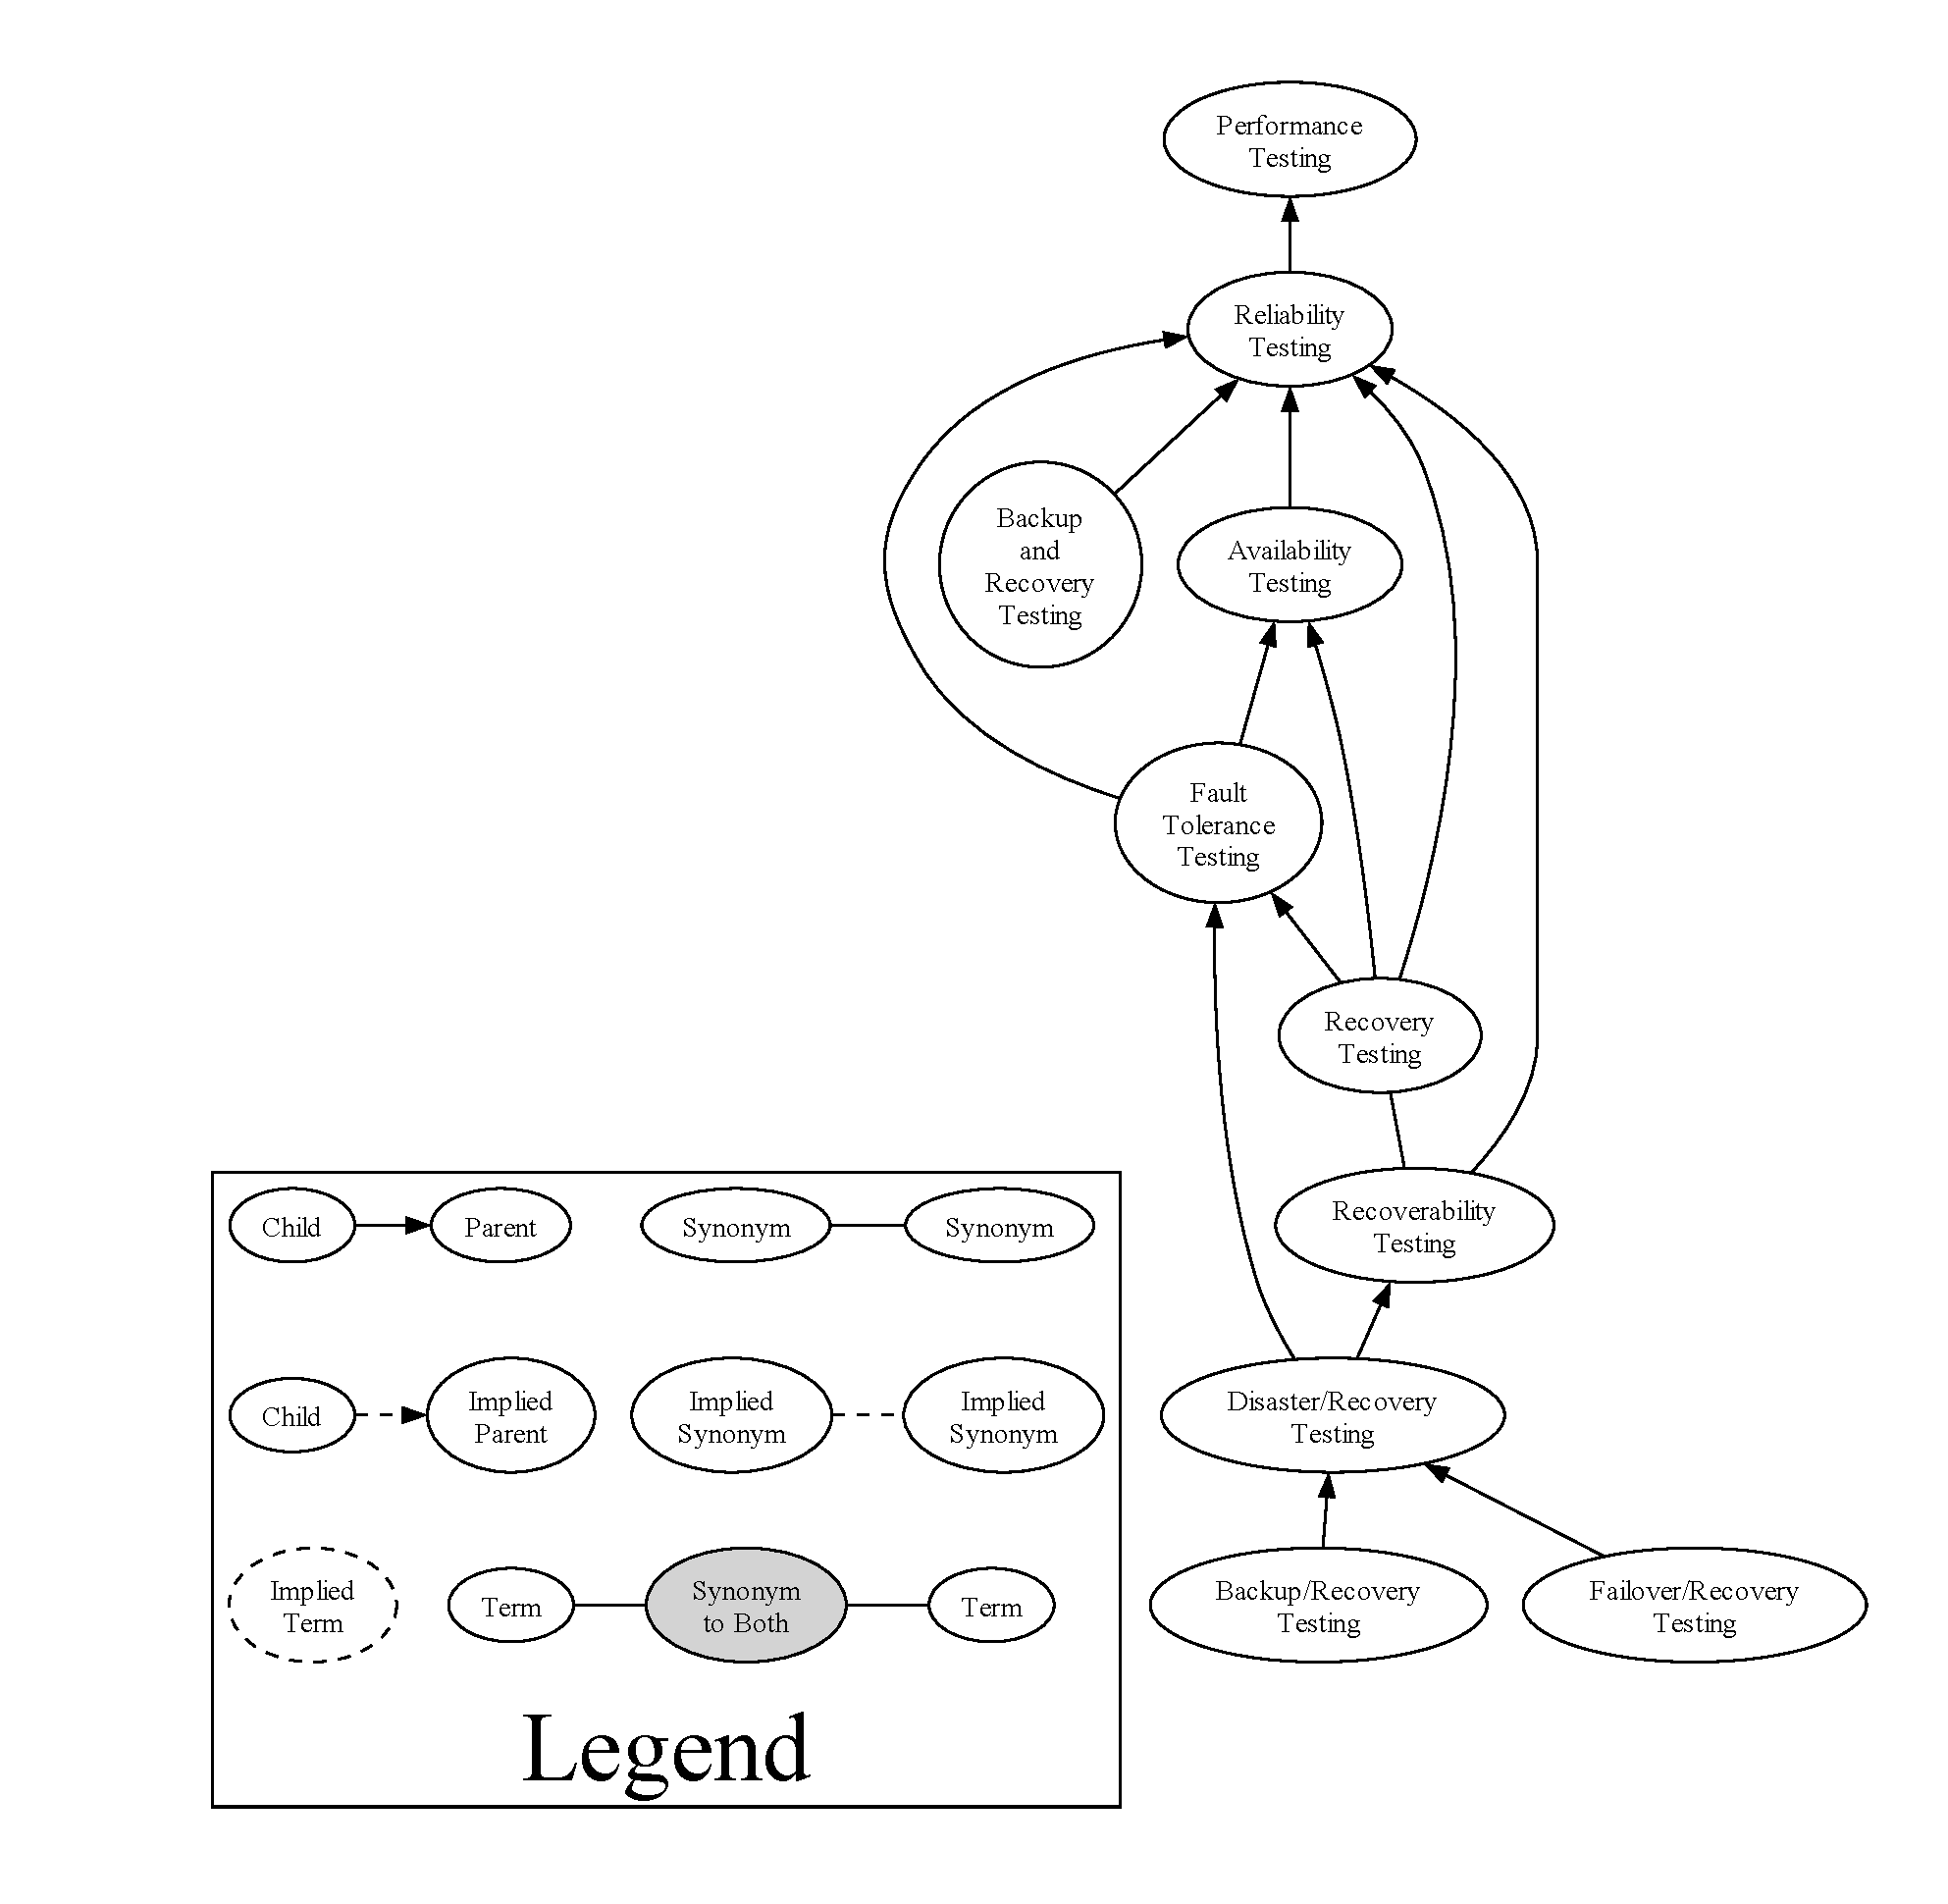
\includegraphics[width=\linewidth]{assets/graphs/recoveryGraph.pdf}}
\newcommand{\recoveryGraphProposed}{
    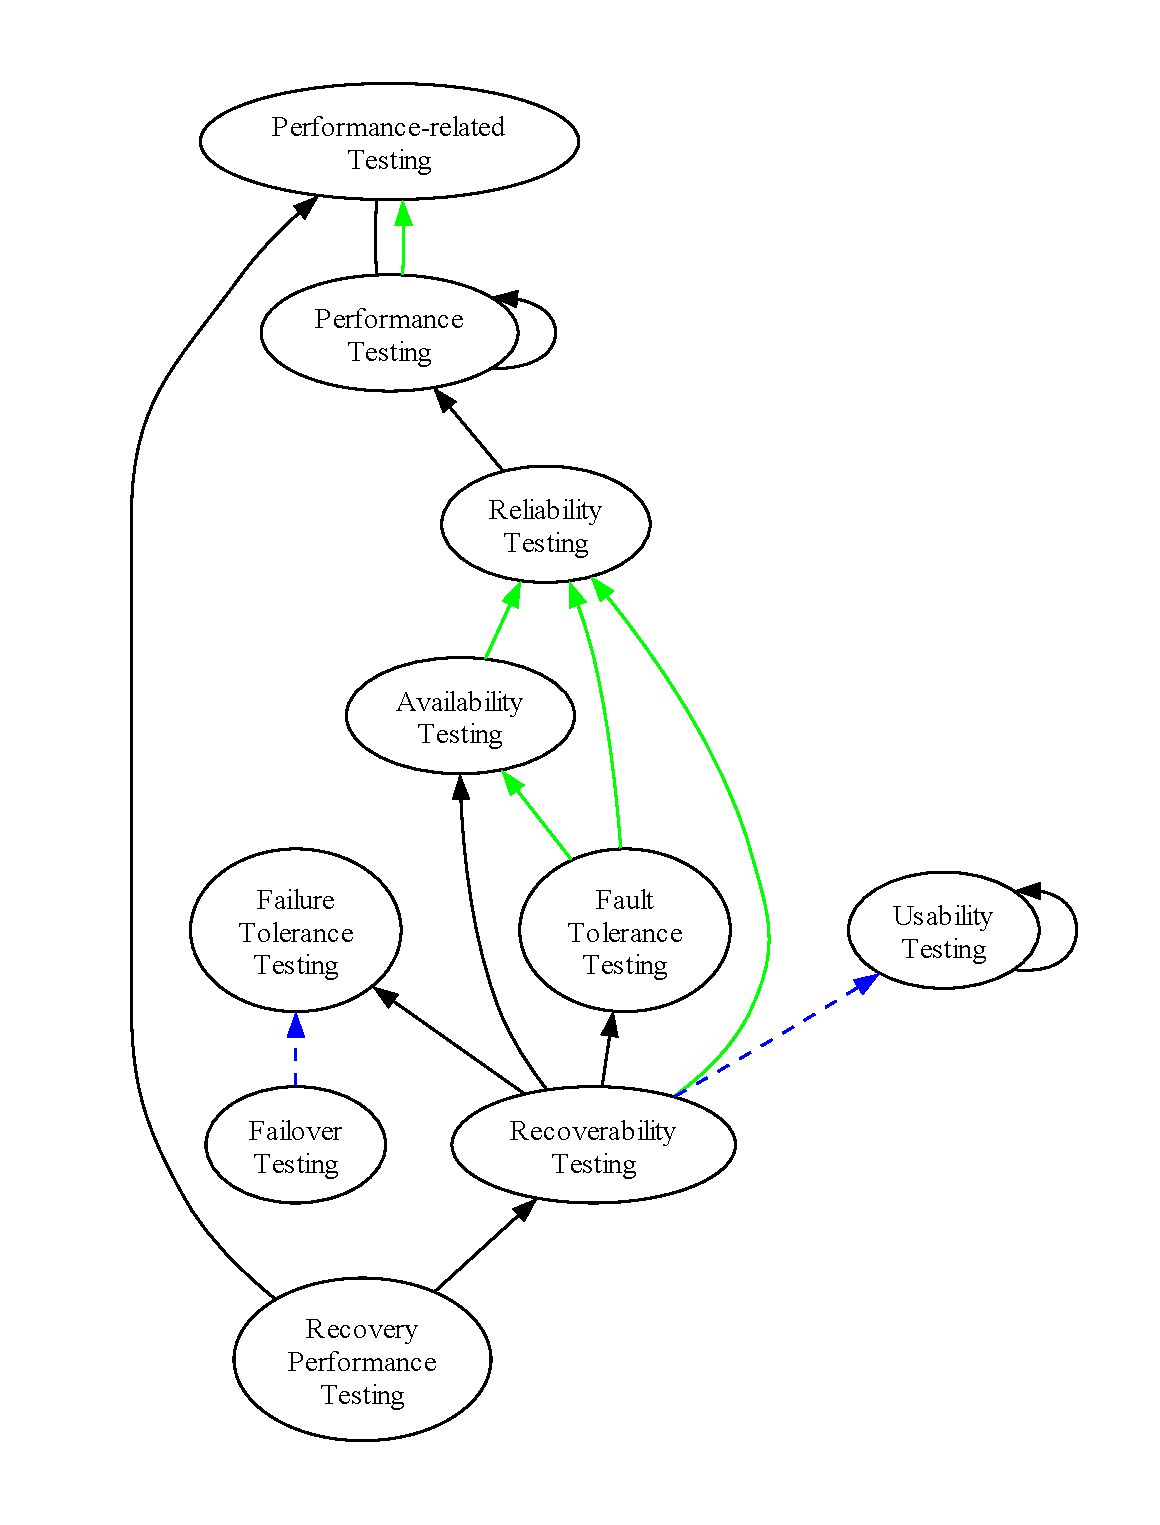
\includegraphics[width=\linewidth]{assets/graphs/recoveryProposedGraph.pdf}
    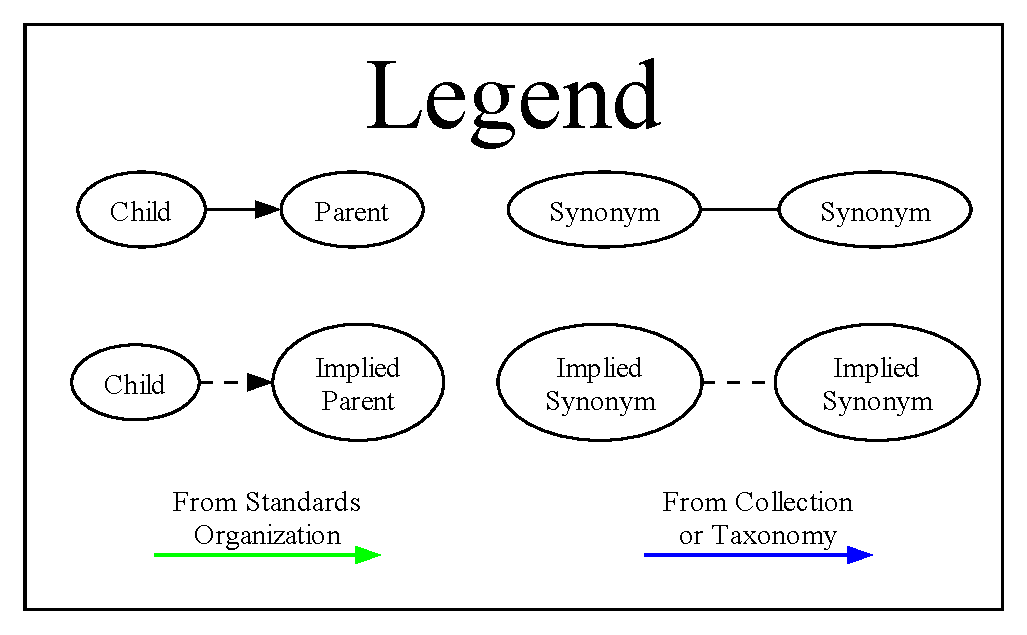
\includegraphics[width=\linewidth]{assets/graphs/manual/manualLegendGreenBlue.pdf}
}

\newcommand{\scalabilityGraphCurrent}{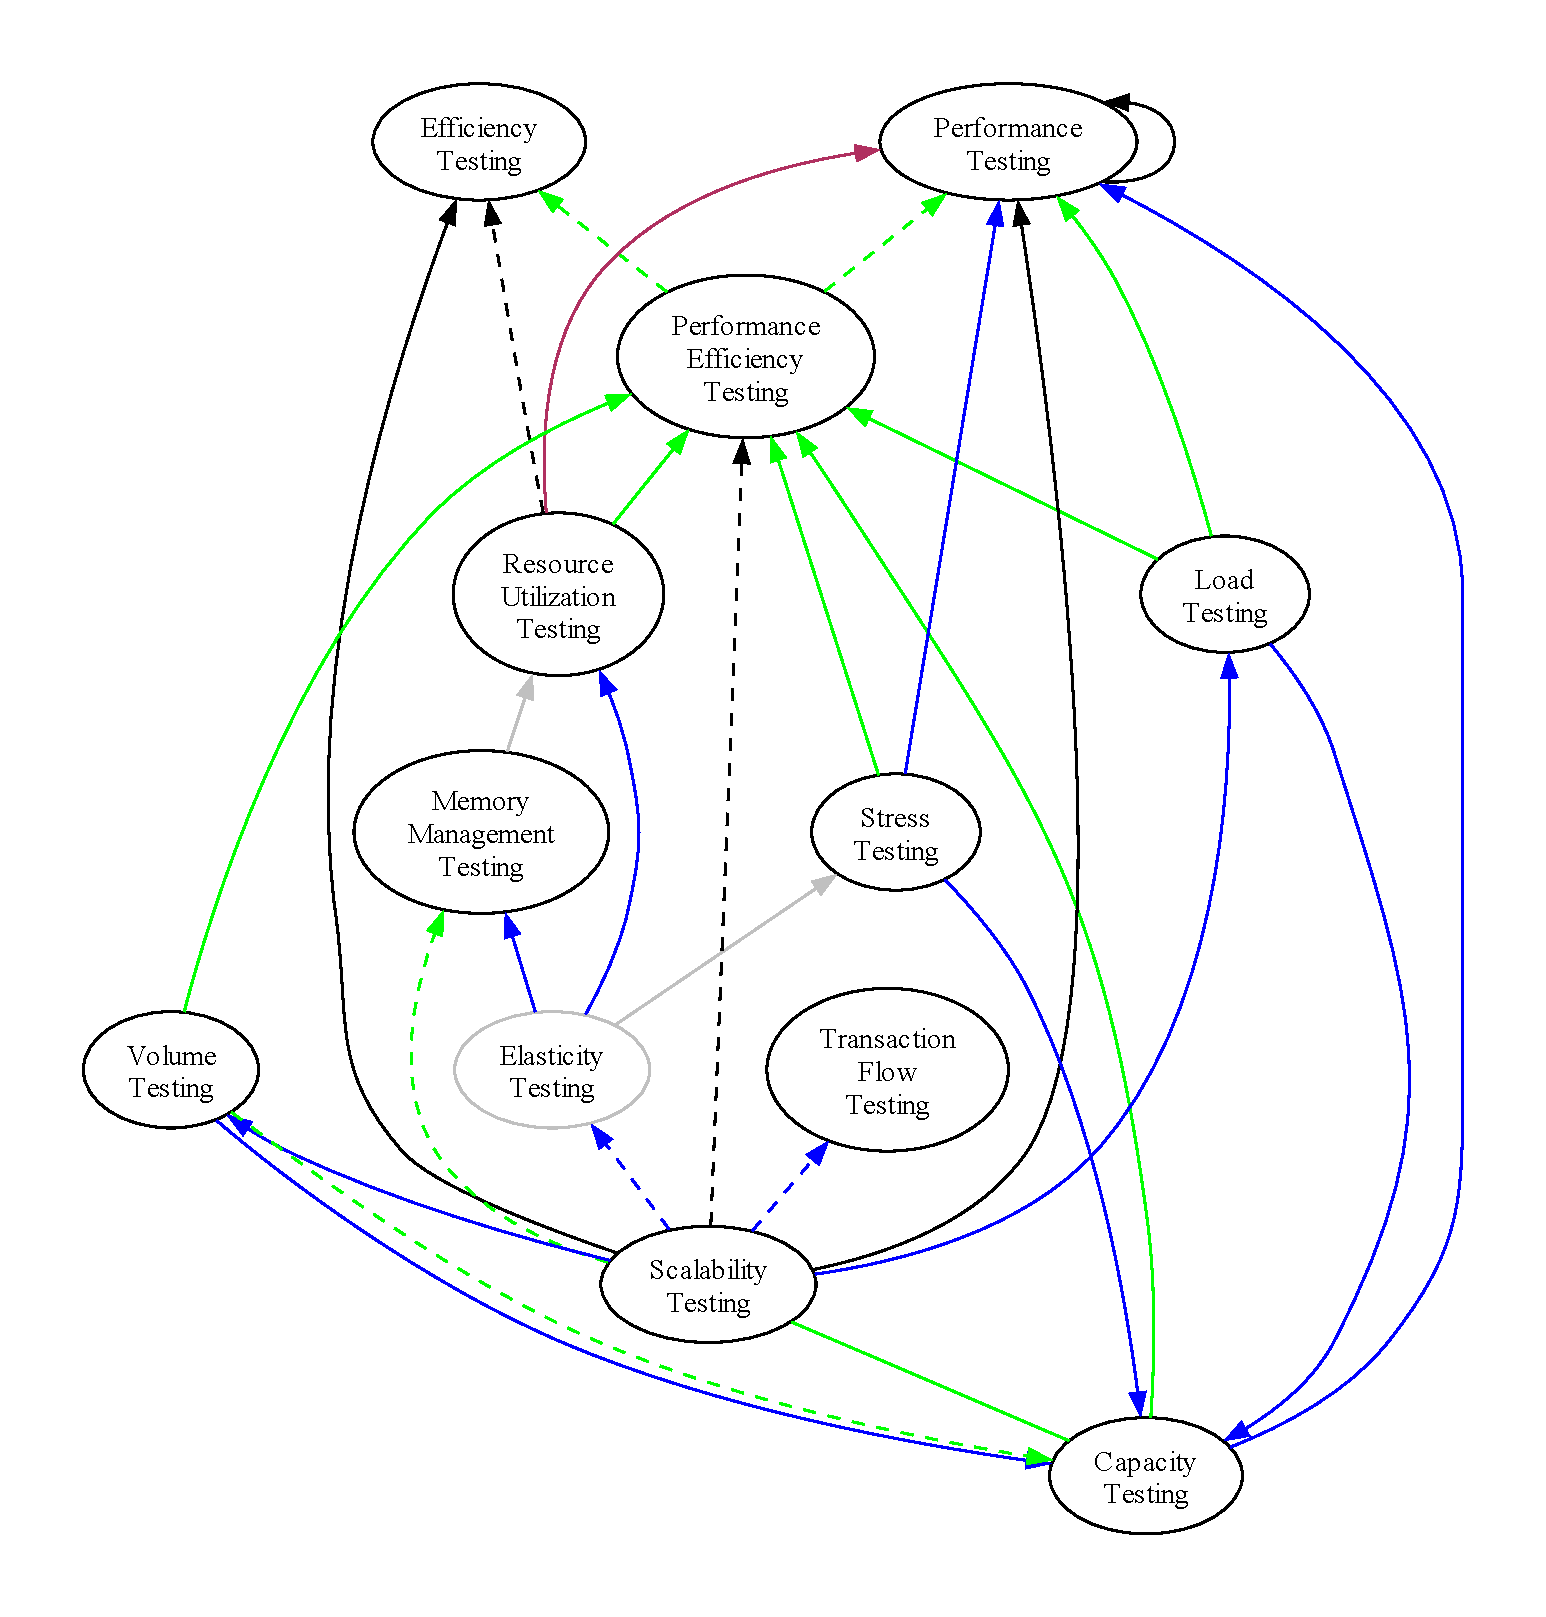
\includegraphics[width=\linewidth]{assets/graphs/scalabilityGraph.pdf}}
\newcommand{\scalabilityGraphProposed}{
    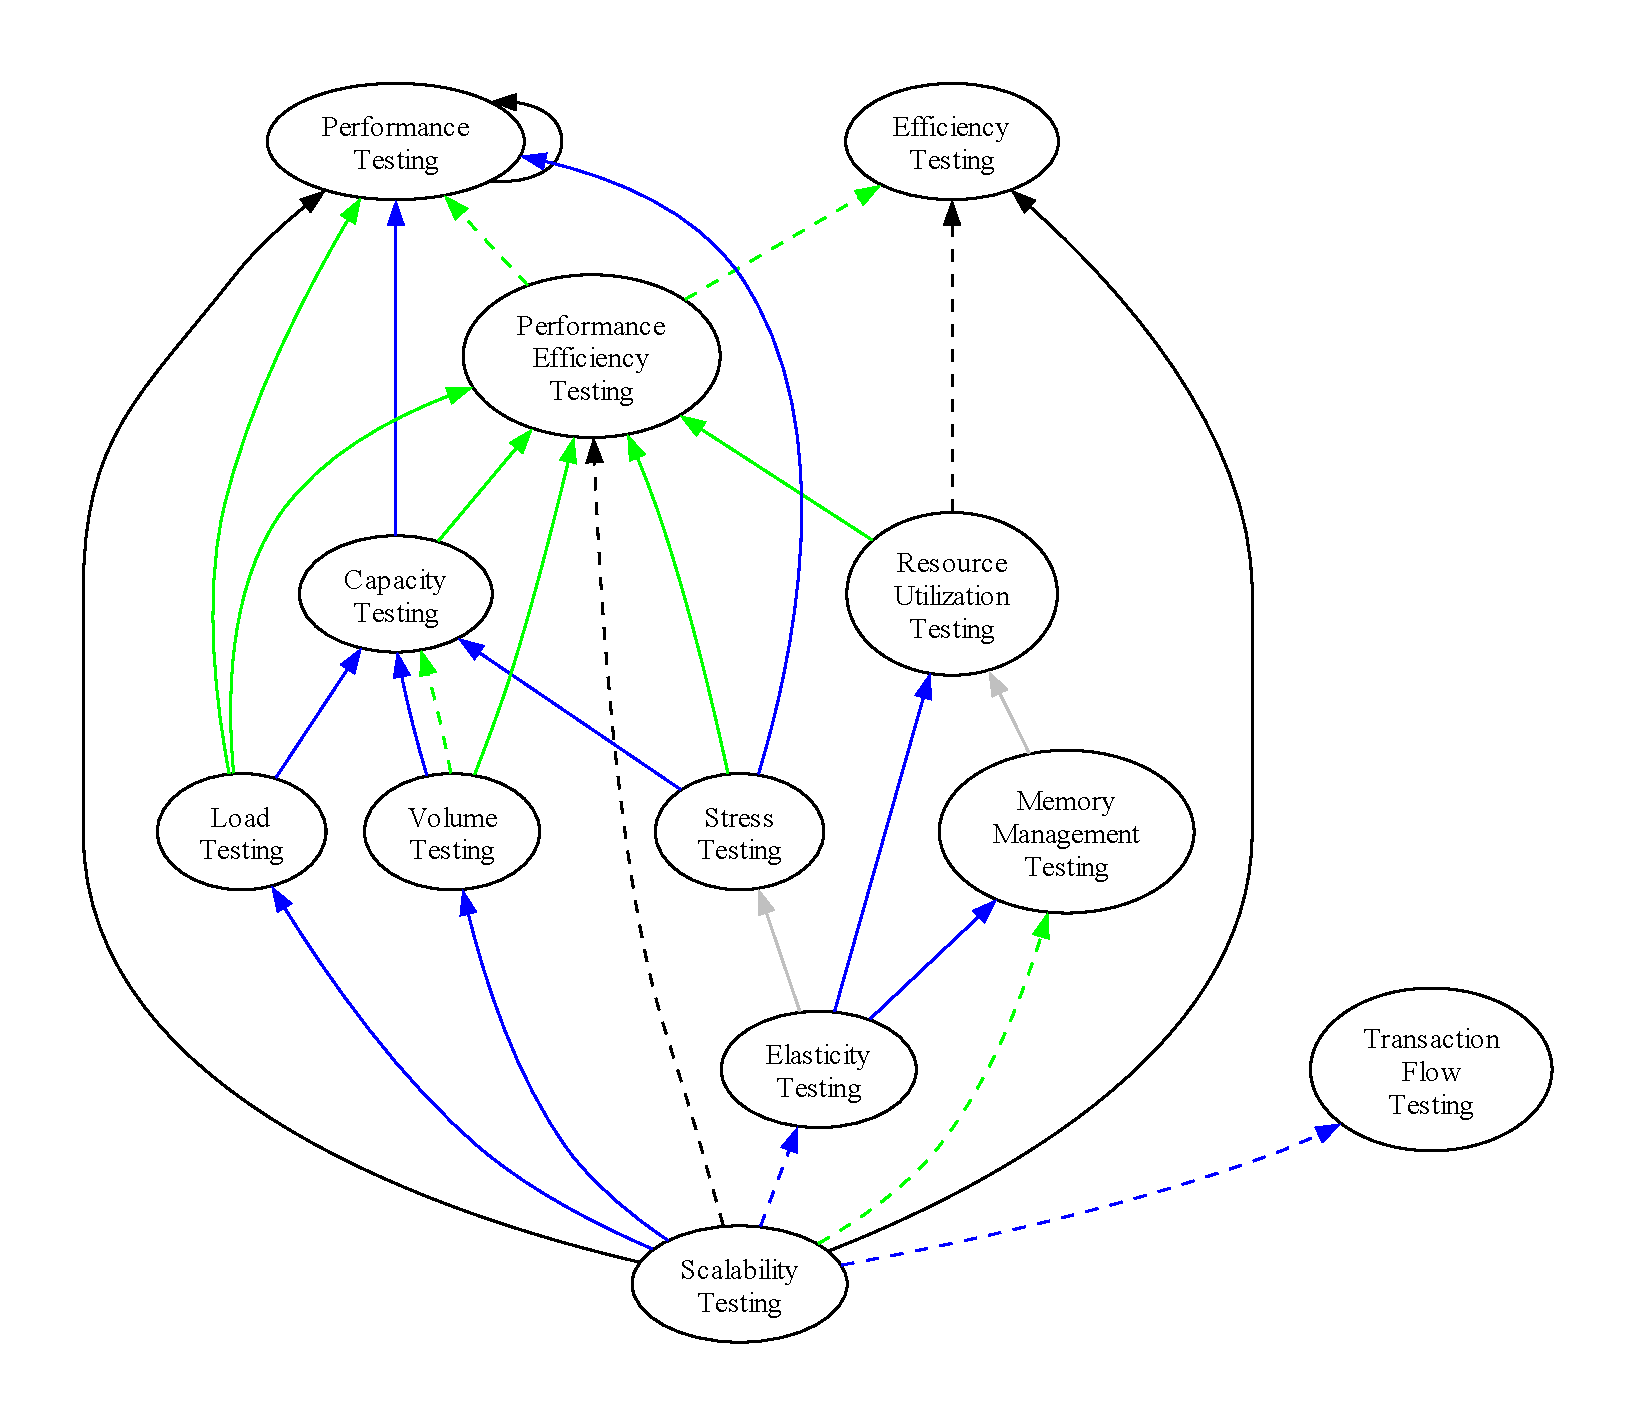
\includegraphics[width=\linewidth]{assets/graphs/scalabilityProposedGraph.pdf}
    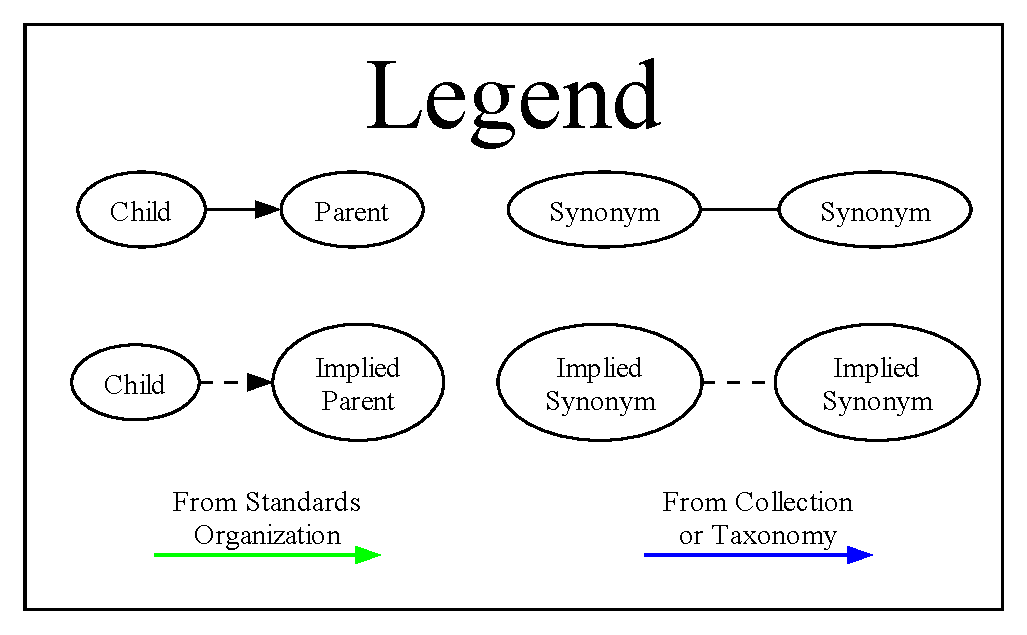
\includegraphics[width=\linewidth]{assets/graphs/manual/manualLegendGreenBlue.pdf}
}

%------------------------------------------------------------------------------
% Images & Figures
%------------------------------------------------------------------------------

\newcommand{\drasilLogo}{assets/images/drasil_logo.png}
\newcommand{\drasilLogoImg}{\begin{figure}[H]
    \centering
    \caption{Drasil's Logo}
    \label{fig:drasilLogo}

    \includegraphics[width=0.6\linewidth]{\drasilLogo}
\end{figure}
}
\newcommand{\refDrasilLogoImg}{\Cref{fig:drasilLogo}}

%------------------------------------------------------------------------------
% Tables
%------------------------------------------------------------------------------

% Organization of files
\newcommand{\organizationTable}{\begin{longtable}[c]{|>{\raggedright}p{0.3\linewidth}|>{\raggedright\arraybackslash}p{0.54\linewidth}|}
    \caption{Template Organization}
    \label{tab:organization}                                              \\

    \hline

    \rowcolor{McMasterMediumGrey}
    \textbf{File/Folder}     & \textbf{Intended Usage \& Description}
    \\ \hline

    \texttt{thesis.tex} & Focal \LaTeX{} file that collects everything and is
    used to build your thesis/report document.
    \\ \hline

    \texttt{Makefile} & A basic \texttt{Makefile} configuration. See
    \texttt{make help} for a list of helpful commands. \\ \hline

    \texttt{build/} & When you build your \acs{pdf}, this folder is used as the
    working directory of LuaLaTeX. Using this allows us to quickly get rid of
    \LaTeX{} build files that can cause problems when we re-build documents. \\
    \hline

    \texttt{manifest.tex} & Basic options that you should certainly configure
    according to your needs.
    \\ \hline

    \texttt{chapters.tex} & All chapters of your thesis should be included here.
    \\ \hline

    \texttt{chapters/} & Enumeration of the chapters of your thesis. I prefer
    using a two-digit indexing pattern for the prefix of file names so that I
    can quickly open up by chapter number using VS Codium. \\ \hline

    \texttt{assets.tex} & Enumeration of the various kinds of ``assets'' in the
    \texttt{assets/} folder. See the file for examples on how you can write your
    extra utility macros. \\ \hline

    \texttt{assets/} & Enumeration of various kinds of ``assets,'' with
    subdirectories for images and figures, tables, and code snippets. \\ \hline

    \texttt{front.tex} & All front matter of your thesis should be included
    here. \\ \hline

    \texttt{front/} & Enumeration of the front chapters of your thesis. These
    chapters should all be numbered using Roman numerals. \\ \hline

    \texttt{back.tex} & All back matter of your thesis should be included here.
    \\ \hline

    \texttt{back/} & Enumeration of the back matter content.
    \\ \hline

    \texttt{acronyms.tex} & List of acronyms you intend to use in your thesis.
    This uses the ``acro'' \LaTeX{} package.
    \\ \hline

    \texttt{macros.tex} & Helpful macros!
    \\ \hline

    \texttt{unicode\_chars.tex} & At times, you might find issues with unicode
    characters, especially in verbatim environments, where you might need to
    manually define them using other font glyphs.
    \\ \hline

    \texttt{mcmaster\_colours.tex} & Macros for the McMaster colour palette.
    \\ \hline

    \texttt{README.md} & Read it!
    \\ \hline

    \texttt{.gitignore} & List of files in the working directory that should be
    ignored by git.
    \\ \hline

    \texttt{latexmkrc} & Used for setting the timezone for latexmk, but can be
    used for other options.
    \\ \hline
\end{longtable}
}

\newcommand{\ieeeTestTermsTable}{% makecell with new lines so VS Code doesn't freak out
\newcommand{\techniqueCell}{\makecell{(Design)\\Technique}}
\newcommand{\levelCell}{\makecell{Level\tablefootnote{\procLevel{\citep}.}\\
        (sometimes\\``Phase''\tablefootnote{``Test phase'' can be a synonym for
            ``test level'' (\citealp[p.~469]{IEEE2017};
            \citeyear[p.~9]{IEEE2013}) but \phaseDef{\citep}})}}

\begin{table}[hbtp!]
    \centering
    \caption{IEEE Testing Terminology}
    \label{tab:ieeeTestTerms}
    % m{0.145\linewidth}
    \begin{tabularx}{\linewidth}{|c|X|m{0.275\linewidth}|}
        \hline
        \rowcolor{McMasterMediumGrey}
        \thead{Term}                      & \thead{Definition}                      & \thead{Examples} \\
        \hline
        Approach                          & A ``high-level test
        implementation choice, typically made as part of the test strategy
        design activity'' that includes ``test level, test type, test technique,
        test practice and the form of static testing to be used''
        \citep[p.~10]{IEEE2022}; described by a \emph{test strategy}
        \citep[p.~472]{IEEE2017} and is also used to ``pick the particular test case
        values'' \citep[p.~465]{IEEE2017} & black or white box, minimum and maximum
        boundary value testing \citep[p.~465]{IEEE2017}                                                \\
        \techniqueCell{}                  & A ``defined'' and ``systematic''
        \citep[p.~464]{IEEE2017} ``procedure used to
        create or select a test model, identify test
        coverage items, and derive corresponding test cases''
        (\citealp[p.~11]{IEEE2022}; similar in \citealp[p.~467]{IEEE2017});
        ``a variety \dots is typically
        required to suitably cover any system'' \citep[p.~33]{IEEE2022} and is
        ``often selected based on team skills and familiarity,
        on the format of the test basis'', and on expectations
        \citep[p.~23]{IEEE2022}           & equivalence partitioning,
        boundary value analysis, branch testing \citep[p.~11]{IEEE2022}                                \\
        \levelCell{}                      & A stage of testing
        ``typically associated with the achievement of particular objectives
        and used to treat particular risks'' \citep[p.~12]{IEEE2022} with
        ``its own documentation and resources'' \citep[p.~469]{IEEE2017}; more
        generally, ``designat[es] \dots the coverage and detail''
        \citep[p.~249]{IEEE2017}          & unit/component testing,
        integration testing, system testing (\citealp[p.~12]{IEEE2022};
        \citealp[p.~467]{IEEE2017})                                                                    \\
        Practice                          & A ``conceptual framework
        that can be applied to \dots [a] test process to facilitate testing''
        (\citealp[p.~14]{IEEE2022}; \citealp[p.~471]{IEEE2017}; OG IEEE 2013);
        more generally, a ``specific type of activity
        that contributes to the execution of a process''
        \citep[p.~331]{IEEE2017}          & scripted testing,
        exploratory testing, automated testing \citep[p.~20]{IEEE2022}                                 \\
        Type                              & ``Testing that is focused
        on specific quality characteristics''
        (\citealp[p.~15]{IEEE2022}; \citealp[p.~473]{IEEE2017};
        OG IEEE 2013)                     & security testing, usability testing,
        performance testing (\citealp[p.~15]{IEEE2022};
        \citealp[p.~473]{IEEE2017})                                                                    \\
        \hline
    \end{tabularx}
\end{table}
}
\newcommand{\otherTestTermsTable}{% Defined here so VS Code doesn't freak out
\def\ieeeEquiv{\makecell{IEEE\\Equivalent}}
\def\swebokLevel{\makecell{Level\\(objective-\\based)\footnote{
            See \discrepref{stage-level-syns}.}}}

\begin{paperTable}
    \centering
    \caption{Other Testing Terminology}
    \label{tab:otherTestTerms}
    \begin{minipage}{\linewidth}
        % Converted from tabularx with help from ChatGPT
        \begin{tabular}{|>{\centering}m{0.08\linewidth}|m{0.4\linewidth}|m{0.3\linewidth}|c|}
            \hline
            \thead{Term}                           & \thead{Definition}           & \thead{Examples} & \thead{\ieeeEquiv{}} \\
            \hline
            % Guidance                               & none given
            % \citep[p.~3]{BarbosaEtAl2006}          & none given         & Technique?                              \\
            \swebokLevel{}                         & Test levels based on the
            purpose of testing \citep[p.~5\=/6]{SWEBOK2024} that ``determine how the test suite is
            identified \dots\ regarding its consistency \dots\ and its composition''
            \citetext{p.~5\=/2}                    &
            conformance testing, installation testing,
            % reliability testing,
            regression testing, performance testing, security testing
            \citep[pp.~5\=/7 to 5\=/9]{SWEBOK2024} & Type?                                                                  \\
            % Method                                 & none given
            % \citep[p.~3]{BarbosaEtAl2006}          & none given         & Practice?                               \\
            Phase                                  & none given
            %(\citealp[p.~221]{Perry2006}; \citealp[p.~3]{BarbosaEtAl2006})  
                                                   & unit testing,
            integration testing, system testing, regression testing (\citealp[p.~221]{Perry2006};
            \citealp[p.~3]{BarbosaEtAl2006})       & Level                                                                  \\
            Procedure                              & The basis for how
            testing is performed that guides the process; ``categorized in[to] testing methods,
            testing guidances\footnote{Testing methods and guidances are omitted from this table
                since \citet{BarbosaEtAl2006} do not define or give examples of them.} and testing techniques''
            \citep[p.~3]{BarbosaEtAl2006}          & none given
            generally; see ``Technique''           & Approach                                                               \\
            Process                                & ``A sequence of
            testing steps'' \citep[p.~2]{BarbosaEtAl2006} ``based on a development technology and \dots\
            paradigm, as well as on a testing procedure''
            \citetext{p.~3}                        & none given                   & Practice                                \\
            Stage                                  & An
            alternative to the ``traditional \dots\ test stages''\footnote{See ``Level'' in
                \Cref{tab:ieeeTestTerms}.} based on ``clear technical groupings''
            \citep[p.~13]{Gerrard2000a}            & desktop development testing,
            infrastructure testing,
            % system testing, large scale integration, and
            post-deployment monitoring
            \citep[p.~13]{Gerrard2000a}            & Level                                                                  \\
            Technique                              & ``Systematic
            procedures and approaches for generating or selecting the most suitable test
            suites'' \citep[p.~5\=/10]{SWEBOK2024} ``on a sound theoretical basis''
            \citep[p.~3]{BarbosaEtAl2006}          & specification-based testing,
            structure-based testing, fault-based testing\footnote{Synonyms for
                these examples are used by \citet[p.~3; OG Mathur, 2012]{SouzaEtAl2017}
                and \citet[p.~3]{BarbosaEtAl2006}.}
            % , experience-based testing, usage-based testing
            (\citealp[pp.~5\=/10, 5\=/13 to 5\=/15]{SWEBOK2024})
            % black-box, white-box, defect/fault-based, model-based testing
            % \citetext{\citealp[p.~3]{SouzaEtAl2017}; OG Mathur, 2012};
            % functional, structural, error-based, state-based testing \citep[p.~3]{BarbosaEtAl2006}
                                                   & Technique                                                              \\
            \hline
        \end{tabular}
    \end{minipage}
\end{paperTable}}

\newcommand{\discrepClssTable}{\begin{paperTable}
    \centering
    \caption{Breakdown of identified \nameref{discrepClasses} by \hyperref[sources]{source category}.}
    \label{tab:discrepClss}
    % \begin{minipage}{\linewidth}
    \begin{spreadtab}{{tabular}{|r|cc|cc|cc|cc|cc|cc|c|}}
        \hline
        @ & @ \multicolumn{2}{c|}{\thead{\nameref{wrong}}} & @ \multicolumn{2}{c|}{\thead{\nameref{miss}}} & @ \multicolumn{2}{c|}{\thead{\nameref{contra}}} & @ \multicolumn{2}{c|}{\thead{\nameref{ambi}}} & @ \multicolumn{2}{c|}{\thead{\nameref{over}}} & @ \multicolumn{2}{c|}{\thead{\nameref{redun}}} & @ \\
        % \cline{2-10}
        @ \thead{\hyperref[sources]{Source Category}} & @ \thead{Exp} & @ \thead{Imp} & @ \thead{Exp} & @ \thead{Imp} & @ \thead{Exp} & @ \thead{Imp} & @ \thead{Exp} & @ \thead{Imp} & @ \thead{Exp} & @ \thead{Imp} & @ \thead{Exp} & @ \thead{Imp} & @ \thead{Total} \\
        \hline
        @ \stds{}   & \stdDiscClsBrkdwn{2}   & \stdDiscClsBrkdwn{3}   & \stdDiscClsBrkdwn{4}   & \stdDiscClsBrkdwn{5}   & \stdDiscClsBrkdwn{6}   & \stdDiscClsBrkdwn{7}   & \stdDiscClsBrkdwn{8}   & \stdDiscClsBrkdwn{9}   & \stdDiscClsBrkdwn{10}   & \stdDiscClsBrkdwn{11}   & \stdDiscClsBrkdwn{12}   & \stdDiscClsBrkdwn{13}   & sum([-12,0]:[-1,0]) \\
        @ \metas{}  & \metaDiscClsBrkdwn{2}  & \metaDiscClsBrkdwn{3}  & \metaDiscClsBrkdwn{4}  & \metaDiscClsBrkdwn{5}  & \metaDiscClsBrkdwn{6}  & \metaDiscClsBrkdwn{7}  & \metaDiscClsBrkdwn{8}  & \metaDiscClsBrkdwn{9}  & \metaDiscClsBrkdwn{10}  & \metaDiscClsBrkdwn{11}  & \metaDiscClsBrkdwn{12}  & \metaDiscClsBrkdwn{13}  & sum([-12,0]:[-1,0]) \\
        @ \texts{}  & \textDiscClsBrkdwn{2}  & \textDiscClsBrkdwn{3}  & \textDiscClsBrkdwn{4}  & \textDiscClsBrkdwn{5}  & \textDiscClsBrkdwn{6}  & \textDiscClsBrkdwn{7}  & \textDiscClsBrkdwn{8}  & \textDiscClsBrkdwn{9}  & \textDiscClsBrkdwn{10}  & \textDiscClsBrkdwn{11}  & \textDiscClsBrkdwn{12}  & \textDiscClsBrkdwn{13}  & sum([-12,0]:[-1,0]) \\
        @ \papers{} & \paperDiscClsBrkdwn{2} & \paperDiscClsBrkdwn{3} & \paperDiscClsBrkdwn{4} & \paperDiscClsBrkdwn{5} & \paperDiscClsBrkdwn{6} & \paperDiscClsBrkdwn{7} & \paperDiscClsBrkdwn{8} & \paperDiscClsBrkdwn{9} & \paperDiscClsBrkdwn{10} & \paperDiscClsBrkdwn{11} & \paperDiscClsBrkdwn{12} & \paperDiscClsBrkdwn{13} & sum([-12,0]:[-1,0]) \\
        \hline
        @ Total & sum([0,-4]:[0,-1]) & sum([0,-4]:[0,-1]) & sum([0,-4]:[0,-1]) & sum([0,-4]:[0,-1]) & sum([0,-4]:[0,-1]) & sum([0,-4]:[0,-1]) & sum([0,-4]:[0,-1]) & sum([0,-4]:[0,-1]) & sum([0,-4]:[0,-1]) & sum([0,-4]:[0,-1]) & sum([0,-4]:[0,-1]) & sum([0,-4]:[0,-1]) & sum([0,-4]:[0,-1]) \\
        \hline
    \end{spreadtab}
    % \end{minipage}
\end{paperTable}
}
\newcommand{\discrepCatsTable}{\begin{paperTable}
    \centering
    \caption{Breakdown of identified \nameref{discrepCategories} by \hyperref[sources]{source category}.}
    \label{tab:discrepCats}
    % \begin{minipage}{\linewidth}
    \begin{spreadtab}[\STsavecell\nSeven{n7}]{{tabularx}{\linewidth}{|s|*{6}{CC|}t|}}
        \hline
        @ & @ \multicolumn{2}{c|}{\thead{\syns{}}} & @ \multicolumn{2}{c|}{\thead{\pars{}}} & @ \multicolumn{2}{c|}{\thead{\cats{}}} & @ \multicolumn{2}{c|}{\thead{\defs{}}} & @ \multicolumn{2}{c|}{\thead{\terms{}}} & @ \multicolumn{2}{c|}{\thead{\srcs{}}} & @ \\
        % \cline{2-10}
        @ \thead{\hyperref[sources]{Source Category}} & @ \thead{Exp} & @ \thead{Imp} & @ \thead{Exp} & @ \thead{Imp} & @ \thead{Exp} & @ \thead{Imp} & @ \thead{Exp} & @ \thead{Imp} & @ \thead{Exp} & @ \thead{Imp} & @ \thead{Exp} & @ \thead{Imp} & @ \thead{Total} \\
        \hline
        @ \stds{}   & \stdDiscCatBrkdwn{1}   & \stdDiscCatBrkdwn{2}   & \stdDiscCatBrkdwn{3}   & \stdDiscCatBrkdwn{4}   & \stdDiscCatBrkdwn{5}   & \stdDiscCatBrkdwn{6}   & \stdDiscCatBrkdwn{7}   & \stdDiscCatBrkdwn{8}   & \stdDiscCatBrkdwn{9}   & \stdDiscCatBrkdwn{10}   & \stdDiscCatBrkdwn{11}   & \stdDiscCatBrkdwn{12}   & \stdDiscCatBrkdwn{13}   \\
        @ \metas{}  & \metaDiscCatBrkdwn{1}  & \metaDiscCatBrkdwn{2}  & \metaDiscCatBrkdwn{3}  & \metaDiscCatBrkdwn{4}  & \metaDiscCatBrkdwn{5}  & \metaDiscCatBrkdwn{6}  & \metaDiscCatBrkdwn{7}  & \metaDiscCatBrkdwn{8}  & \metaDiscCatBrkdwn{9}  & \metaDiscCatBrkdwn{10}  & \metaDiscCatBrkdwn{11}  & \metaDiscCatBrkdwn{12}  & \metaDiscCatBrkdwn{13}  \\
        @ \texts{}  & \textDiscCatBrkdwn{1}  & \textDiscCatBrkdwn{2}  & \textDiscCatBrkdwn{3}  & \textDiscCatBrkdwn{4}  & \textDiscCatBrkdwn{5}  & \textDiscCatBrkdwn{6}  & \textDiscCatBrkdwn{7}  & \textDiscCatBrkdwn{8}  & \textDiscCatBrkdwn{9}  & \textDiscCatBrkdwn{10}  & \textDiscCatBrkdwn{11}  & \textDiscCatBrkdwn{12}  & \textDiscCatBrkdwn{13}  \\
        @ \papers{} & \paperDiscCatBrkdwn{1} & \paperDiscCatBrkdwn{2} & \paperDiscCatBrkdwn{3} & \paperDiscCatBrkdwn{4} & \paperDiscCatBrkdwn{5} & \paperDiscCatBrkdwn{6} & \paperDiscCatBrkdwn{7} & \paperDiscCatBrkdwn{8} & \paperDiscCatBrkdwn{9} & \paperDiscCatBrkdwn{10} & \paperDiscCatBrkdwn{11} & \paperDiscCatBrkdwn{12} & \paperDiscCatBrkdwn{13} \\
        \hline
        @ Total & sum([0,-4]:[0,-1]) & sum([0,-4]:[0,-1]) & sum([0,-4]:[0,-1]) & sum([0,-4]:[0,-1]) & sum([0,-4]:[0,-1]) & sum([0,-4]:[0,-1]) & sum([0,-4]:[0,-1]) & sum([0,-4]:[0,-1]) & sum([0,-4]:[0,-1]) & sum([0,-4]:[0,-1]) & sum([0,-4]:[0,-1]) & sum([0,-4]:[0,-1]) & sum([0,-4]:[0,-1]) \\
        \hline
    \end{spreadtab}
    % \end{minipage}
\end{paperTable}

% From https://tex.stackexchange.com/a/248135/192195
\laterdef{totalDiscreps}{\nSeven{}}}

\newcommand{\testReqsTable}{% To prevent VSCode from aligning things weirdly
\def\typeHead{Testing\\Approach}

\begin{table}[hbtp!]
    \centering
    \caption{Testing Requirements}
    \label{tab:testReqs}
    \begin{tabularx}{\textwidth}{|p{0.14\textwidth}|X|c|c|}
        \hline
        \rowcolor{McMasterMediumGrey}
        \thead{\typeHead}       & \thead{Requirements}                         & \thead{In Drasil?} & \thead{Addable?} \\
        \hline
        Unit testing            & Code modules and their specifications        & ??                 & ??               \\
        Integration testing     & Code modules and their interfaces            & ??                 & ??               \\
        System testing          & Requirements specification; most of the code
                                & ??                                           & ??                                    \\
        Acceptance testing      & Customer requirements and feedback           & ??                 & ??               \\
        Installation testing    & Algorithm for installation; environments to
        test in; method to check
        successful installation & ??                                           & ??                                    \\
        \hline
    \end{tabularx}
\end{table}}
